\documentclass[aspectratio=169,11pt]{beamer}

\usepackage[utf8]{inputenc}
\usepackage{graphicx}
\usepackage{tikz}
\usepackage{anyfontsize}
\usetheme{Boadilla}
\usecolortheme{dolphin}

\definecolor{PrismNavy}{RGB}{25,49,75}
\definecolor{PrismTeal}{RGB}{0,119,126}
\definecolor{PrismMist}{RGB}{235,244,245}
\definecolor{PrismGold}{RGB}{220,157,45}

\setbeamercolor{normal text}{fg=PrismNavy,bg=white}
\setbeamercolor{structure}{fg=PrismTeal}
\setbeamercolor{frametitle}{fg=white,bg=PrismNavy}
\setbeamercolor{framesubtitle}{fg=PrismTeal,bg=white}
\setbeamercolor{title}{fg=white,bg=PrismNavy}
\setbeamercolor{subtitle}{fg=white}
\setbeamercolor{block title}{fg=white,bg=PrismTeal}
\setbeamercolor{block body}{fg=PrismNavy,bg=PrismMist}
\setbeamercolor{itemize item}{fg=PrismGold}
\setbeamercolor{author in head/foot}{fg=PrismNavy,bg=PrismMist}
\setbeamercolor{date in head/foot}{fg=white,bg=PrismNavy}
\setbeamerfont{title}{size=\LARGE,series=\bfseries}
\setbeamerfont{frametitle}{size=\large,series=\bfseries}
\setbeamerfont{framesubtitle}{size=\small}
\setbeamerfont{author}{size=\large,series=\bfseries}
\setbeamerfont{institute}{size=\normalsize}
\setbeamertemplate{navigation symbols}{}
\setbeamertemplate{frametitle}[default][center]
\setbeamertemplate{blocks}[rounded][shadow=false]
\setbeamertemplate{footline}{%
  \leavevmode%
  \hbox{%
    \begin{beamercolorbox}[wd=0.78\paperwidth,ht=2.5ex,dp=1ex,leftskip=1em]{author in head/foot}%
      \scriptsize Grupo 5 \textcolor{PrismTeal}{\textbullet} Etanol--benzeno
    \end{beamercolorbox}%
    \begin{beamercolorbox}[wd=0.22\paperwidth,ht=2.5ex,dp=1ex,center]{date in head/foot}%
      \scriptsize \insertframenumber/\inserttotalframenumber
    \end{beamercolorbox}%
  }%
}
\setbeamertemplate{title page}{%
  \begin{tikzpicture}[remember picture,overlay]
    \fill[PrismNavy] (current page.south west) rectangle (current page.north east);
    \begin{scope}[shift={(current page.south west)},x=\paperwidth,y=\paperheight]
      \fill[PrismTeal] (0.74,0) rectangle (1,1);
      \fill[PrismGold] (0.07,0.745) rectangle (0.14,0.752);
      \node[anchor=north west,text=PrismMist,inner sep=0,font=\small\bfseries]
        at (0.07,0.88) {TERMODINÂMICA II};
      \node[anchor=north west,text=white,inner sep=0,align=left,
        font=\fontsize{29}{34}\selectfont\bfseries]
        at (0.07,0.67) {Equilíbrio\\líquido--vapor};
      \node[anchor=north west,text=PrismMist,inner sep=0,align=left,font=\large]
        at (0.07,0.365) {Etanol (1) + benzeno (2)};
      \node[anchor=north west,text=PrismMist,inner sep=0,font=\small]
        at (0.07,0.29) {Modelo de Van Laar};
      \draw[white,opacity=0.25,line width=0.4pt] (0.07,0.20) -- (0.67,0.20);
      \node[anchor=north west,text=PrismGold,inner sep=0,font=\small\bfseries]
        at (0.07,0.145) {\insertauthor};
      \node[anchor=north west,text=white,inner sep=0,font=\small]
        at (0.07,0.095) {\insertinstitute};
      \node[text=white,opacity=0.85,font=\scriptsize\bfseries,align=center]
        at (0.87,0.77) {SISTEMA BINÁRIO};
      \node[text=white,font=\fontsize{34}{38}\selectfont\bfseries]
        at (0.87,0.59) {ELV};
      \draw[PrismGold,line width=1pt] (0.80,0.48) -- (0.94,0.48);
      \node[text=white,font=\Large\bfseries] at (0.87,0.36) {1 atm};
      \node[text=white,opacity=0.85,font=\scriptsize,align=center]
        at (0.87,0.28) {PRESSÃO DO SISTEMA};
    \end{scope}
  \end{tikzpicture}%
}

\title{Equilíbrio Líquido--Vapor}
\subtitle{Etanol (1) + benzeno (2) a 1 atm}
\author[Grupo 5]{Grupo 5}
\institute{Hycaro, Mariana e Osvaldino}
\date{}

\begin{document}

\begin{frame}[plain]
  \titlepage
\end{frame}

\begin{frame}{Gráficos: não idealidade da fase líquida}
  \framesubtitle{Modelo de Van Laar a $73{,}55\,^{\circ}\mathrm{C}$}
  \begin{columns}[T,onlytextwidth]
    \begin{column}{0.49\textwidth}
      \centering
      \begin{beamercolorbox}[wd=\linewidth,sep=0.3em,center,rounded=true]{block body}
        \textbf{Figura 1 — Coeficientes de atividade}\\[0.2em]
        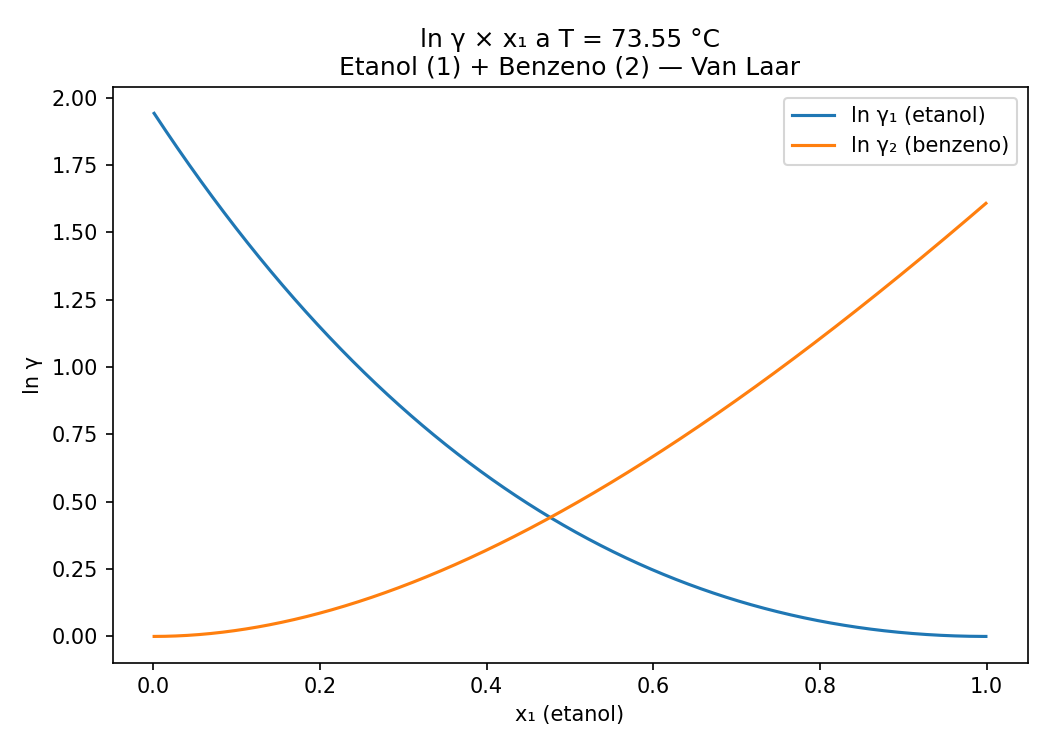
\includegraphics[width=\linewidth,height=0.52\textheight,keepaspectratio]{1_ln_gamma.png}
      \end{beamercolorbox}
      \vspace{-0.1em}
      \scriptsize $\ln\gamma_1$ e $\ln\gamma_2$ positivos no interior da mistura: desvio positivo da lei de Raoult.\\
      Nos limites de diluição infinita: $\gamma_1^{\infty}\approx7$ e $\gamma_2^{\infty}\approx5$.
    \end{column}
    \begin{column}{0.49\textwidth}
      \centering
      \begin{beamercolorbox}[wd=\linewidth,sep=0.3em,center,rounded=true]{block body}
        \textbf{Figura 2 — Energia de Gibbs em excesso}\\[0.2em]
        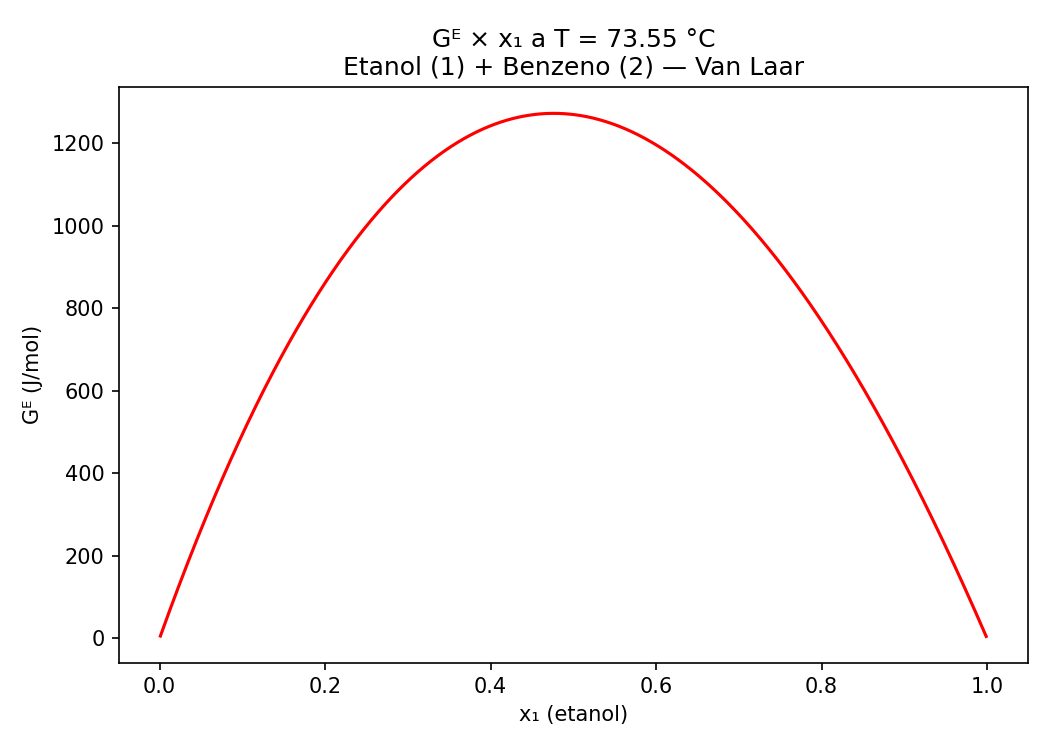
\includegraphics[width=\linewidth,height=0.52\textheight,keepaspectratio]{2_GE.png}
      \end{beamercolorbox}
      \vspace{-0.1em}
      \scriptsize $G^E$ é zero nos componentes puros e positivo nas misturas.\\
      Máximo: $1{,}273\,\mathrm{J/mol}$ em $x_1\approx0{,}476$. O gráfico mostra $G^E$, não $G^E/RT$.
    \end{column}
  \end{columns}
\end{frame}

\begin{frame}{Gráficos: equilíbrio líquido--vapor}
  \framesubtitle{A 1 atm}
  \begin{columns}[T,onlytextwidth]
    \begin{column}{0.49\textwidth}
      \centering
      \begin{beamercolorbox}[wd=\linewidth,sep=0.3em,center,rounded=true]{block body}
        \textbf{Figura 3 — Diagrama $T$--$x$--$y$}\\[0.2em]
        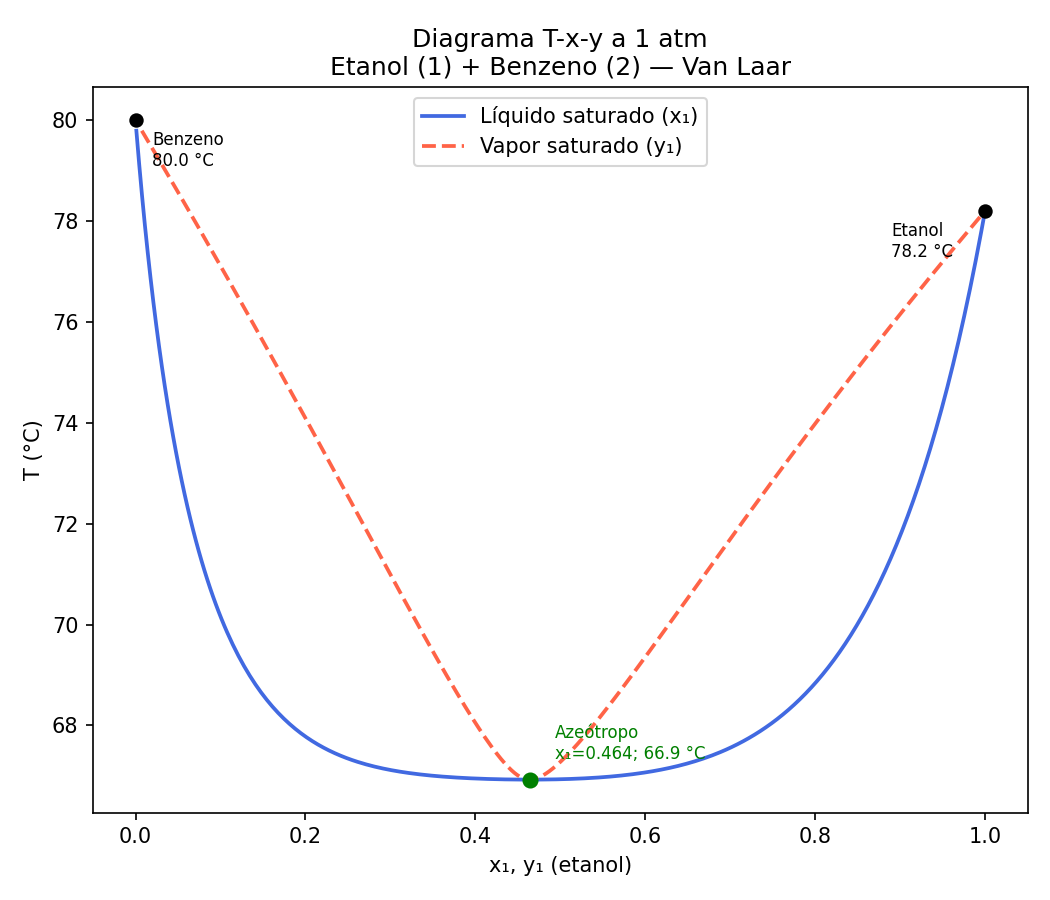
\includegraphics[width=\linewidth,height=0.52\textheight,keepaspectratio]{3_Txy.png}
      \end{beamercolorbox}
      \vspace{-0.1em}
      \scriptsize Curvas de líquido e vapor saturados. O mínimo indica azeótropo de ebulição mínima: $x_1=y_1\approx0{,}464$ a $66{,}93\,^{\circ}\mathrm{C}$.
    \end{column}
    \begin{column}{0.49\textwidth}
      \centering
      \begin{beamercolorbox}[wd=\linewidth,sep=0.3em,center,rounded=true]{block body}
        \textbf{Figura 4 — Diagrama $x$--$y$}\\[0.2em]
        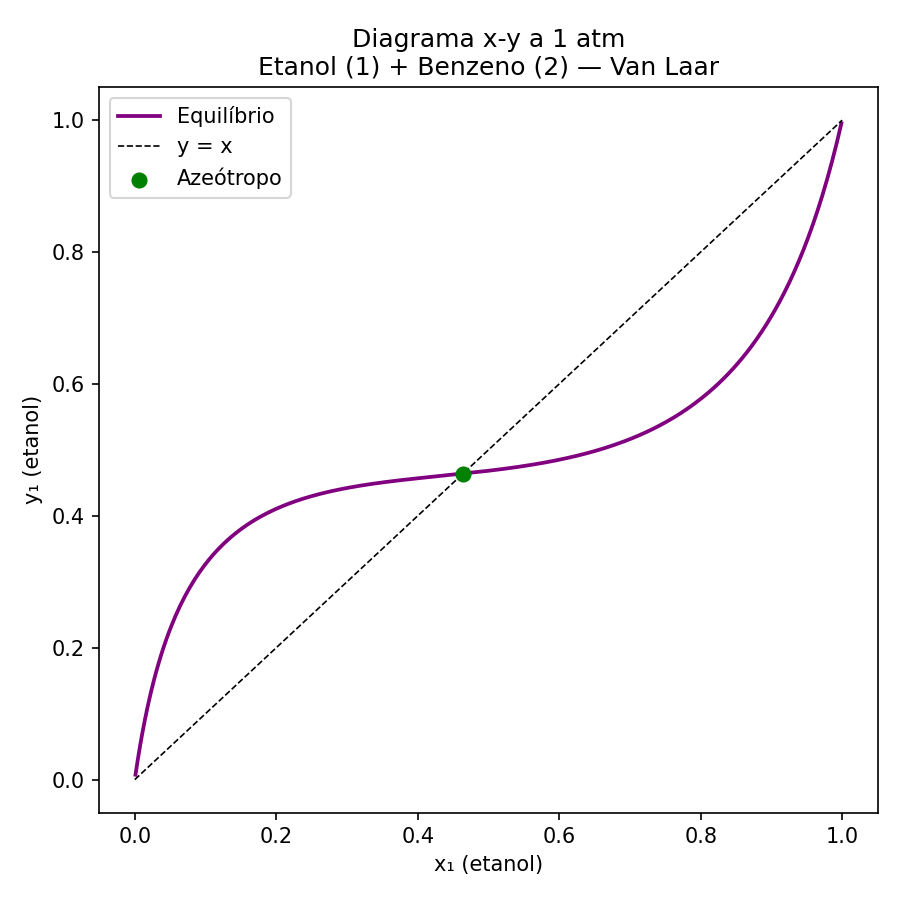
\includegraphics[width=\linewidth,height=0.52\textheight,keepaspectratio]{4_xy.png}
      \end{beamercolorbox}
      \vspace{-0.1em}
      \scriptsize A curva cruza $y_1=x_1$ no azeótropo. Abaixo dele, $y_1>x_1$; acima, $y_1<x_1$. Em $x_1=y_1$, a destilação simples não altera a composição.
    \end{column}
  \end{columns}
\end{frame}

\begin{frame}{Aplicação profissional: unidade de recuperação de solventes}
  \framesubtitle{Exemplo de decisão de processo}
  \begin{block}{Onde e para quê}
    Em uma unidade de recuperação de solventes de uma indústria química ou petroquímica, a equipe recebe uma corrente com etanol e benzeno e avalia se uma coluna de destilação a 1 atm consegue recuperar o etanol na pureza especificada.
  \end{block}
  \begin{itemize}
    \item O diagrama $T$--$x$--$y$ estima a temperatura de operação; o diagrama $x$--$y$ mostra quanto etanol passa ao vapor em cada estágio.
    \item O azeótropo calculado ($x_1\approx0{,}464$) é o limite: a destilação simples não consegue atravessar essa composição.
    \item Se a especificação exigir ultrapassá-lo, o engenheiro deve avaliar outra rota de separação e os controles de segurança para o benzeno [6].
  \end{itemize}
\end{frame}

\begin{frame}{Referências}
  \scriptsize
  \begin{enumerate}
    \setlength{\itemsep}{0.35em}
    \item Smith, J. M.; Van Ness, H. C.; Abbott, M. M. \textit{Introduction to Chemical Engineering Thermodynamics}. 7. ed. McGraw-Hill, 2005. (Antoine e Van Laar.)
    \item Prausnitz, J. M.; Lichtenthaler, R. N.; Azevedo, E. G. \textit{Molecular Thermodynamics of Fluid-Phase Equilibria}. 3. ed. Prentice Hall, 1999.
    \item NIST. \textit{Chemistry WebBook}, SRD 69: registros de etanol e benzeno.
    \item CRC. \textit{Handbook of Chemistry and Physics}, seção “Azeotropic Data of Binary Mixtures”.
    \item Tiesinga, E. et al. CODATA recommended values of the fundamental physical constants: 2018. \textit{Rev. Mod. Phys.}, 93, 025010, 2021. DOI: 10.1103/RevModPhys.93.025010.
    \item National Toxicology Program. \textit{15th Report on Carcinogens: Benzene}. 2021.
    \item Tabela de grupos da disciplina, Grupo 5: parâmetros de Van Laar e faixa de temperatura.
  \end{enumerate}
\end{frame}

\end{document}
